\documentclass{article}

\usepackage[margin=1in]{geometry}
\usepackage{amssymb}
\usepackage{tikz}
\usetikzlibrary{positioning}

\title{Interaction Diagram - Add Version Simplified}
\author{Adam Hammes}

% no page number at bottom
\pagenumbering{gobble}

\begin{document}
\maketitle

\begin{center}
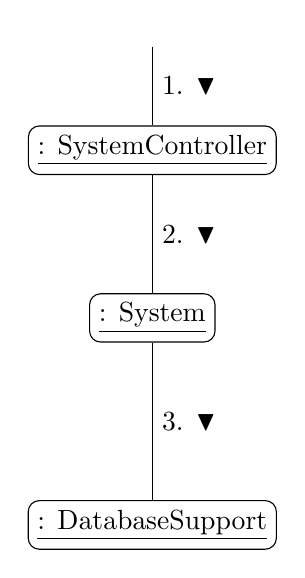
\begin{tikzpicture}[
  auto,
  block/.style = {
    rectangle,
    draw=black,
    align=center,
    rounded corners
  }
]

\node[] (start)  {};

\node[block, below = of start]         (controller) {\underline{: SystemController}};
\node[block, below = 1.5of controller] (system)     {\underline{: System}};
\node[block, below = 2cm of system]    (database)   {\underline{: DatabaseSupport}};

\draw (start)      -- (controller) node[midway] {1. $\blacktriangledown$};
\draw (controller) -- (system)     node[midway] {2. $\blacktriangledown$};
\draw (system) -- (database)     node[midway]   {3. $\blacktriangledown$};

\end{tikzpicture}

\vspace{0.5cm}

\begin{enumerate}
  \item \texttt{b:=addVersion(uid:String, bid:String, path:String, type:String):boolean}
  \item \texttt{b:=addVersion(uid:String, bid:String, path:String, type:String):boolean}
  \item \texttt{b:=addVersion(uid:String, bid:String, path:String, type:String):boolean}
\end{enumerate}
\end{center}

\end{document}
